% vim: set tw=78 tabstop=4 shiftwidth=4 aw ai:

\chapter{Implementarea infrastructurilor rețelelor Peer-to-Peer cu ajutorul
virtualizării}
\label{chapter:virt-infra}

Considerând protocoalele și aplicațiile de rețea, două tipuri de medii
sunt în general folosite pentru testare, măsurare și analiză: configurații
de laborator și experimentele aplicate în lumea reală. Configurațiile
de laborator sau experimentale sunt configurații adaptate evaluării
unor protocoale; în acest caz, experimentatorul deține controlul
complet asupra mediului. Acesta este de obicei cazul testării
funcționalității sau experimente în care experimentatorul necesită controlul
complet asupra procesului. Experimentatorul poate folosi o infrastructură
de laborator, una bazată pe sisteme cluster/cloud sau o infrastructură
oferită de către comunitate, cum ar fi 
PlanetLab\footnote{\url{http://www.planet-lab.org/}}. Rias~\cite{rias} este
un exemplu de topologie overlay creată peste o infrastructură PlanetLab.

\section{Soluții de virtualizare}
\label{sec:virt-infra:openvz}

Un ,,buzzword'' important în ultimul deceniu, tehnologia de virtualizare
a evoluat de la bazele teoretice puse la sfârșitul anilor '70 către o
diversitate de implementări mature în ziua de astăzi. Odată cu creșterea
capacității hard-disk-urilor, a memoriei și a puterii de procesare
(în cea mai mare parte în număr de core-uri), soluțiile de virtualizare
au ajuns să furnizeze cel mai bun mod de alocare a resurselor. Noi
tehnologii precum virtualizarea hardware, îmbunătățirile I/O sau migrarea
în timp real au sporit cererea pentru soluții de virtualizare eficiente
care consolidează resursele hardware din prezent și viitor.

\subsection{Beneficiile aduse de virtualizare}

Soluțiile de virtualizare și-au găsit locul în utilizările de zi cu zi
datorită faptului că aduc beneficii importante, în special în ceea ce
privește costurile. Un sistem fizic dat poate în acest caz rula diverse
instanțe de sistem de operare, în timp ce în absența virtualizării ar fi
necesare mai multe sisteme.

Se pot identifica~\cite{best-damn-virt} trei trei beneficii importante ale
virtualizării:

\begin{itemize}
  \item consolidare;
  \item fiabilitate;
  \item securitate.
\end{itemize}

\textbf{Consolidarea}, un aspect important în special în cadrul mediului
de afaceri, permite ,,unificarea'' resurselor deasupra unui număr mic
de platforme fizice. Viteza sporită a procesoarelor și a subsistemului I/O
și capacitatea memoriei aflată în continuă creștere, toate acestea pot
fi acum folosite pentru a furniza suficiente resurse pentru multiple
sisteme de operare virtualizate. ,,Data center''-urile moderne trebuie
să fie active chiar și atunci când nu se rulează nimic util, fapt ce
duce la risipirea infrastructurii. Folosirea soluțiilor de virtualizare și
a tehnicilor de migrare permite unificarea serverelor virtuale multiple
peste un hardware partajat.

Soluțiile de virtualizare oferă \textbf{fiabilitate} prin izolare. Un
eveniment de eșec pe o mașină virtuală nu va afecta o altă mașină virtuală.
,,Partiționarea'' întrebuințată de către soluțiile de virtualizare se
referă la faptul că fiecare mașină virtuală rulează pe un hardware simulat
dedicat și specializat. Izolarea și partiționarea permit alocarea dinamică
a sistemelor noi oricând este necesar, excluzând nevoia de a achiziționa
hardware suplimentar.

Izolarea oferită de către tehnologiile de virtualizare este un aspect cheie
în ceea ce privește asigurarea securității mașinilor virtuale. În cazul
în care o mașină virtuală eșuează sau este compromisă, acest fapt nu va
afecta alte sisteme și, la nevoie, poate fi dezactivată rapid. Acest
rezultat ar fi foarte dificil de obținut pe o infrastructură fizică.

\subsection{OpenVZ}

Datorită faptului că virtualizarea la nivelul sistemului de operare s-a
dovedit a fi cea mai bună bază pentru construirea unei infrastructuri
Peer-to-Peer, a trebuit să alegem între soluții existente cum ar fi
OpenVZ, LXC sau V-Server. Datorită experienței cu Linux, soluția a trebuit
să fie una bazată pe acesta, astfel că a trebuit să alegem între OpenVZ,
LXC și V-Server. Deși LXC are în prezent avantajul de a fi activ în versiunea
principală a nucleului, în momentul în care am început construirea
infrastructurii acesta era încă într-un stadiu incipient de dezvoltare.
În plus, resursele pentru documentare sunt reduse. Între OpenVZ și V-Server
am ales OpenVZ datorită documentației foarte bune din punct de vedere
calitativ și în urma recomandărilor și a experienței altor utilizatori.

Într-un mod similar cu alte soluții de virtualizare la nivelul sistemului
de operare, OpenVZ este o serie de patch-uri pentru nucleul Linux,
acesta îmbunătățind izolarea resurselor și a proceselor între așa-zisele
containere. Distribuțiile Linux importante vin de obicei cu o versiune
de nucleu care poate rula OpenVZ și care este ușor de instalat. O
serie de unelte din spațiul utilizator permit instalarea și configurarea
mașinilor virtuale. Majoritatea comenzilor și cuvintelor cheie încep cu
prefixul \texttt{vz}.

Fiind o soluție la nivelul sistemului de operare, în care se pot realiza
ușor configurările rețelei și având o interfață flexibilă de configurare
a limitării de resurse, OpenVZ a fost considerată a fi cea mai potrivită
alegere pentru implementarea unei infrastructuri de rețea virtualizată.
Capitolele următoare vor oferi detalii legate de procesul și uneltele
folosite pentru scenariile referitoare la crearea infrastructurii și
respectiv implementarea swarm-ului Peer-to-Peer.

\section{Configurarea infrastructurii Peer-to-Peer virtualizate}
\label{sec:virt-infra:setup}

Crearea unui mediu virtualizat necesită noduri hardware unde vor fi
plasate mașinile virtuale, infrastructura de rețea, un set de șabloane
OpenVZ pentru instalare și un framework care permite comandarea clienților
aflați în mașini virtuale. Fiecare mașină virtuală rulează o aplicație
BitTorrent care a fost instrumentată pentru a folosi o interfață în linie
de comandă ușor de automatizat.

În ciuda limitărilor sale, OpenVZ este cea mai bună alegere pentru crearea
unui mediu virtualizat folosit la evaluarea clienților BitTorrent. 
Penalizările minime de performanță impuse de acesta și consumul mic de 
resurse asigură rularea a zeci de mașini virtuale pe același nod fizic.

\subsection{Privire de ansamblu}
\label{sec:virt-overall}

%The above mentioned values assume the usage of the hrktorrent/libtorrent
%BitTorrent client. They also assume the scheduling impact of all processes in
%the VEs induces low overhead on the overall performance. However, even
%considering the scheduling overhead, a modest system would still be able to
%run at least 10 to 20 VEs.

% TODO: mention virtualization measurements

În urma experimentelor am ajuns la concluzia că un mediu de testare
virtualizat bazat pe OpenVZ ar oferi capabilități de testare similare cu
acelea ale unui cluster non-virtualizat, la cel mult 10\% din cost.
Configurația noastră experimentală formată din doar 10 calculatoare este
capabilă de a rula cel puțin 100 de medii virtuale cu pierderi minime
de performanță.

\begin{figure}
  \begin{center}
    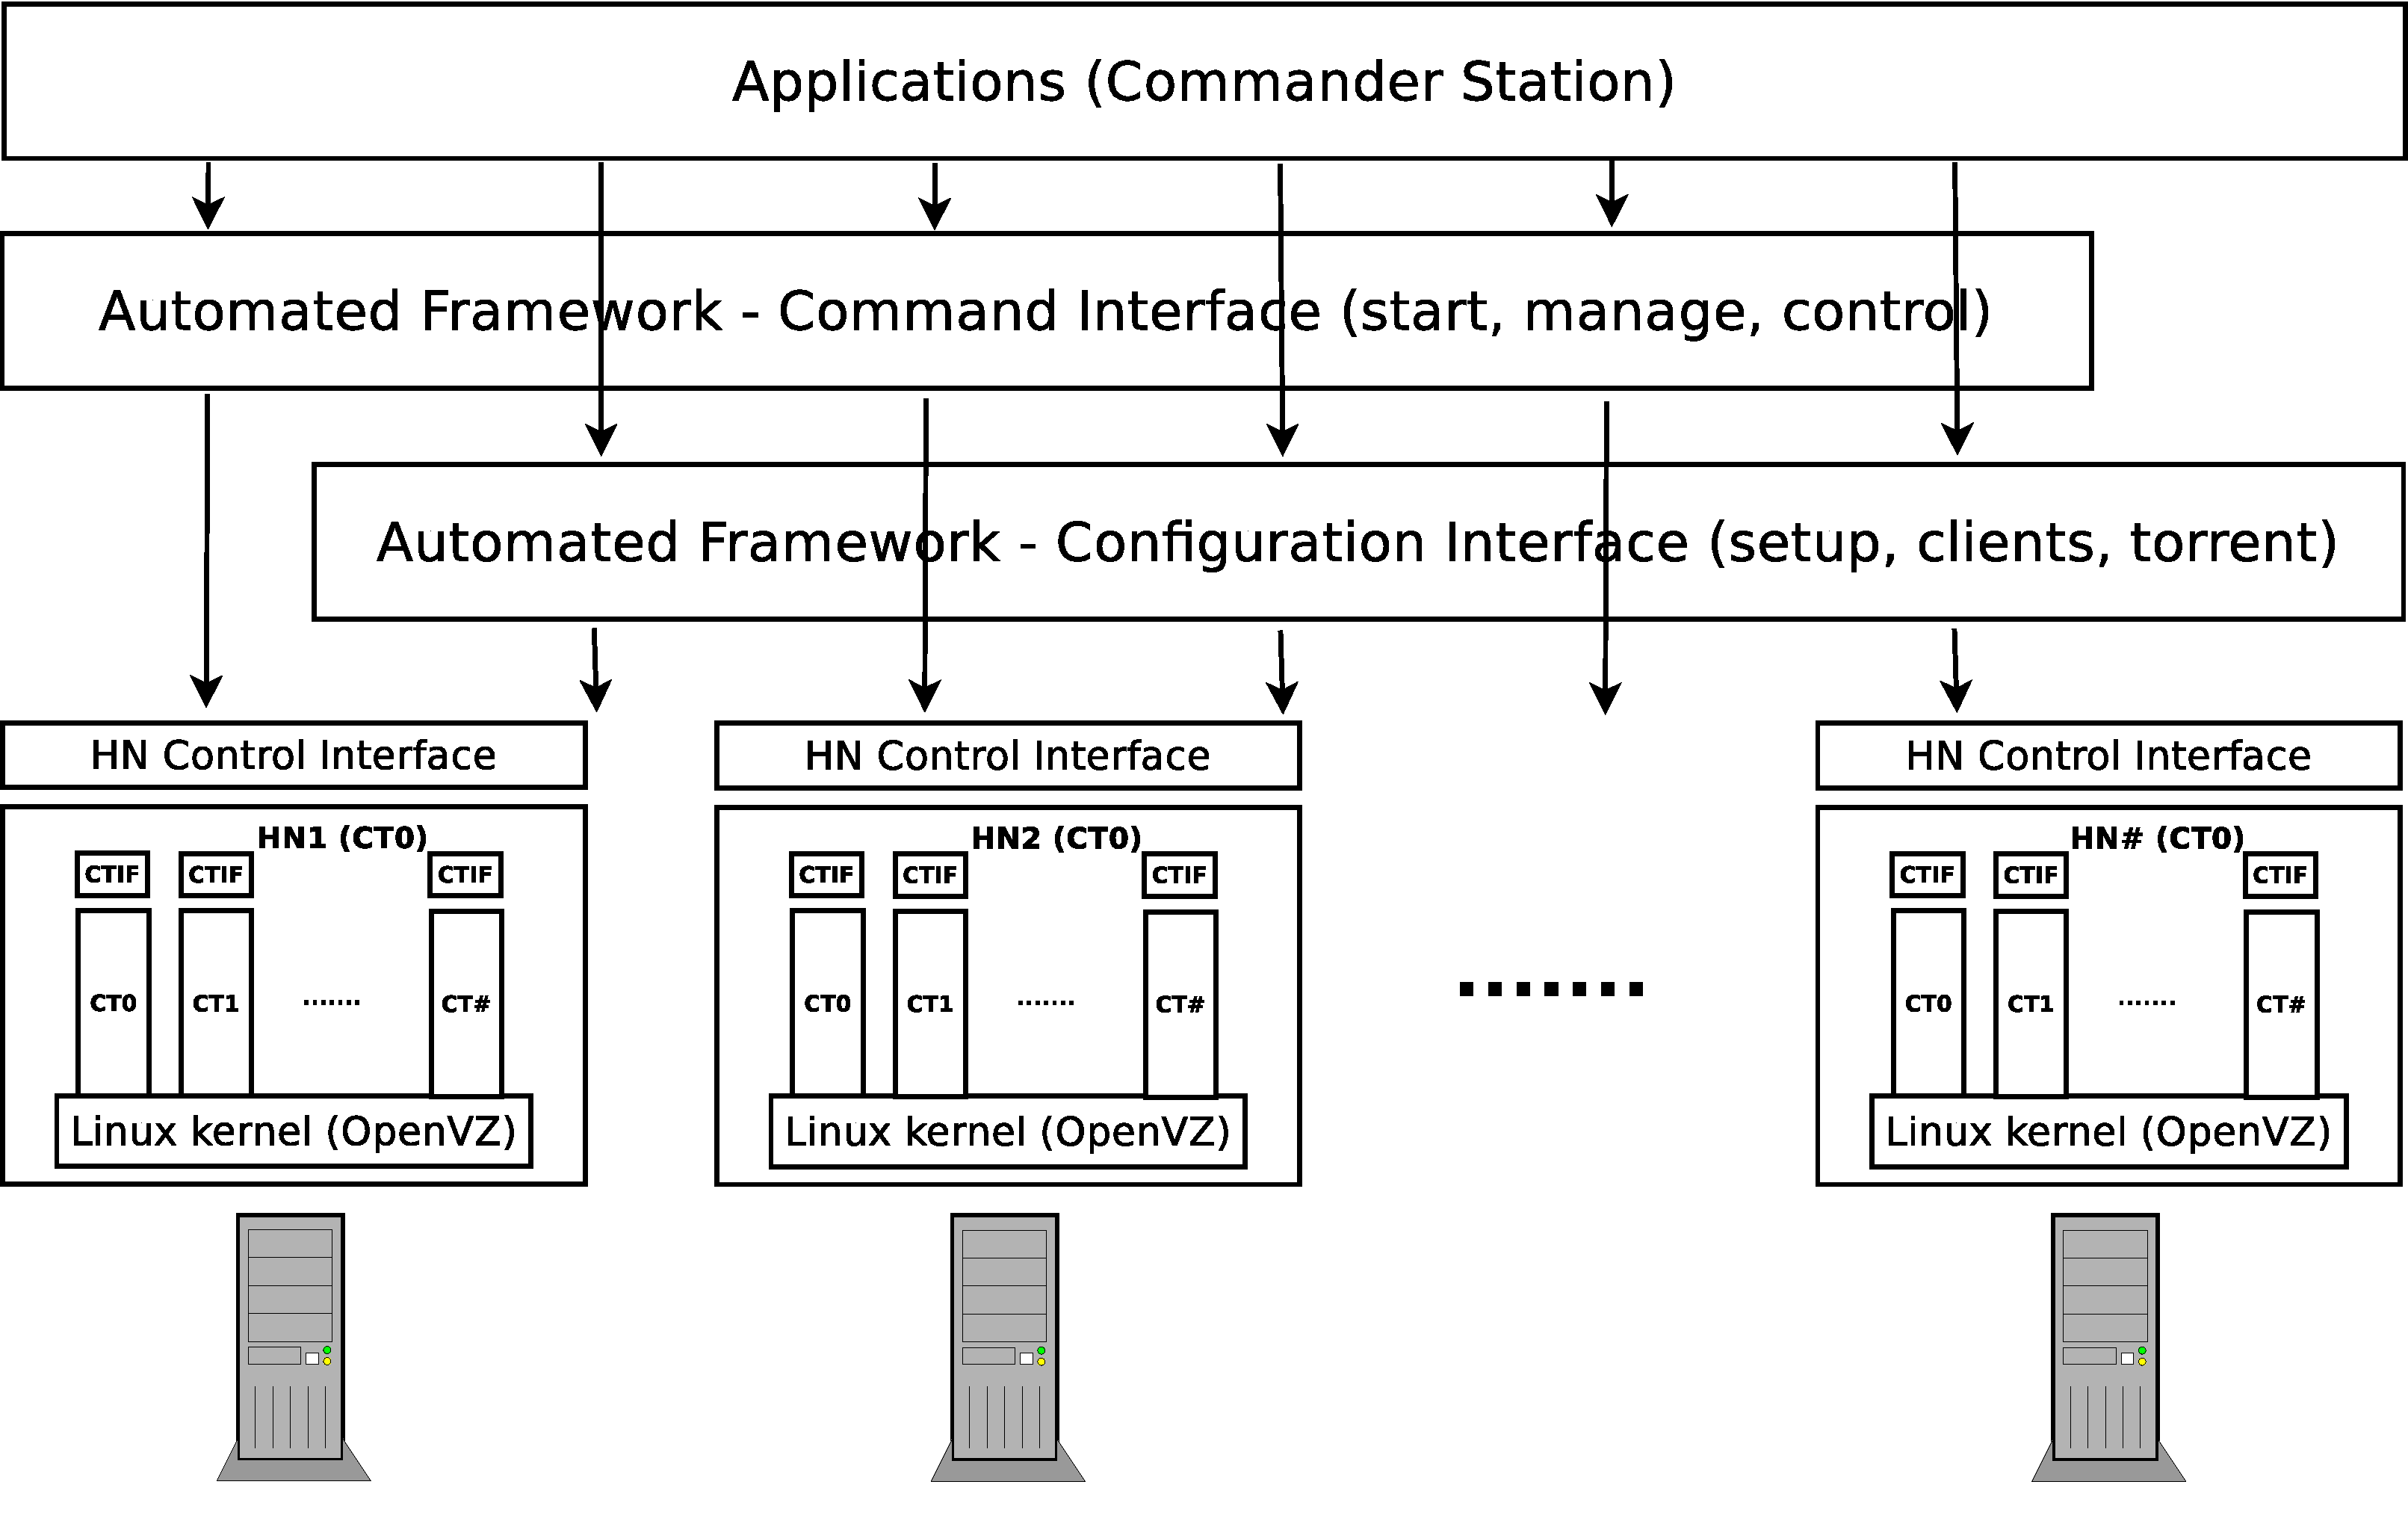
\includegraphics[width=0.7\textwidth]{src/img/virt-infra/virt-infra-overview}
  \end{center}
  \caption{Infrastructura de testare}
  \label{fig:virt-infra:infrastructure-overview}
\end{figure}

Figura~\ref{fig:virt-infra:infrastructure-overview} oferă o privire
de ansamblu asupra infrastructurii de testare BitTorrent.

Infrastructura este proiectată pentru a rula pe sisteme hardware de
consum. Fiecare sistem fizic folosește o implementare de mașină virtuală
OpenVZ pentru a rula sisteme virtuale multiple peste același nod hardware.
Fiecare mașină virtuală conține uneltele de bază pentru rularea și compilarea
clienților BitTorrent. Implementările BitTorrent au fost instrumentate pentru
comenzi automatizate și de asemenea pentru a oferi către ieșire informații
de stare și jurnalizare necesare pentru analiza ulterioară și interpretarea
rezultatelor. Datorită faptului că infrastructura se dorește a fi
independentă de diversele implementări, adăugarea unui nou client BitTorrent
se referă la adăugarea script-urilor și instrumentației necesare.

Mediul virtualizat reprezintă astfel o alternativă mai ieftină și mai
flexibilă la un cluster, cu pierderi foarte mici de performanță.
Dezavantajul principal al acestei abordări este asimetria dintre medii
virtualizate care rulează pe sisteme hardware diferite. Motivul îl
reprezintă discrepanța între lățimea de bandă dintre mediile virtuale
rulând pe același nod hardware și cea dintre mediile virtuale rulând pe
mașini fizice diferite. Această problemă poate fi corectată folosind
limitări de trafic, asigurând astfel o simetrie a lățimii de bandă între
sistemele virtuale.

\section{Evaluarea virtualizării}

În contextul unei multitudini de soluții de virtualizare, o infrastructură
pentru implementarea scenariilor Peer-to-Peer trebuie să ia în considerare
cât de adecvată este fiecare soluție. În urma unor studii empirice am ales
OpenVZ drept soluție potrivită cu nevoile noastre, dar căreia îi lipsește 
o metodă formală de evaluare.

Având în vedere utilizarea soluțiilor de virtualizare pentru scopul nostru,
luăm în considerare trei dimensiuni importante:

\begin{itemize}
  \item \textbf{eficiența} (scalabilitatea) -- cât de multe mașini
  virtuale/containere pot fi implementate pe o gazdă virtuală, permițând
  simularea adecvată a unui mediu;
  \item \textbf{izolarea} -- cât de bine sunt separate resursele mașinilor
  virtuale;
  \item \textbf{fiabilitate} -- cât de multe defecte software au loc pentru
  o soluție dată; acestea pot fi o consecință a implementării sau a
  suprautilizării/abuzului unei resurse.
\end{itemize}

Wood~et~al.~\cite{virt-prof-model} au investigat VMware ESX și Xen și au
creat un model I/O și un profil.

O abordare similară cu a noastră a fost aleasă de 
Soltesz~et~al.~\cite{virt-doppel}. Aceștia au considerat Xen și Linux
Vserver ca fiind reprezentative pentru para-, respectiv pan-virtualizare.
Metricile acestora includ performanța, izolarea și scalabilitatea, cu
semnificații similare cu cele enumerate mai sus.

\textbf{Eficiența} este o măsură legată de implementarea unui număr mare
de mașini virtuale și containere deasupra unui sistem fizic dat.
Padala~et~al.~\cite{eval-virt-performance} au arătat că OpenVZ duce la
o penalizare de performanță mai mică în comparație cu Xen. Cu toate acestea,
nu au fost folosite metode formale iar studiul nu ia în considerare alte
soluții de virtualizare la nivelul SO.

O măsurătoare formală a eficienței/performanței virtualizării trebuie să
ia în calcul trei aspecte:

\begin{itemize}
  \item resursele hardware;
  \item implementarea software-ului (în cazul nostru, implementarea
  clientului BitTorrent);
  \item soluția de virtualizare.
\end{itemize}

Astfel, formalizăm eficiența drept o funcție a celor trei metrici de mai sus:
As such, we formalize efficiency as a function of the three dimensions above:

\begin{align}
Eff & = f(HW, SW, VS)\\
Eff & = f(RAM, HDD, CPU, NET, OS, PS, BT, VS, NVM)\\
Eff &= \frac{VMB}{HNB}
\end{align}

unde:

\begin{multicols}{2}
    \begin{itemize}
      \item \texttt{Eff}: eficiența/performanța
      \item \texttt{HW}: resursele hardware
      \item \texttt{SW}: implementarea software-ului
      \item \texttt{VS}: soluția de virtualizare
      \item \texttt{RAM}: capacitatea memoriei RAM a sistemului
      \item \texttt{HDD}: capacitatea dispozitivului I/O
      \item \texttt{CPU}: viteza procesorului
      \item \texttt{NET}: aspecte legate de rețea
      \item \texttt{OS}: implementarea sistemului de operare
      \item \texttt{PS}: procese de bază ale container-ului
      \item \texttt{BT}: implementarea BitTorrent
      \item \texttt{NVM}: numărul de mașini virtuale
      \item \texttt{VMB}: comportamentul mașinii virtuale
      \item \texttt{HNB}: comportamentul mașinii fizice
    \end{itemize}
\end{multicols}

\textbf{Izolarea} reprezintă un mod de a determina cât de bine este o
mașină virtuală separată în raport cu o altă mașină virtuală și cu sistemul
de bază. Datorită faptului că VE-urile OpenVZ folosesc același nucleu,
este evident că măsura izolării este mai mică decât aceea a Xen sau KVM.
Izolarea servește drept o dimensiune importantă pentru măsurarea a cât
de adecvată este o soluție de virtualizare dată. Abilitatea soluției
în a izola complet o mașină virtuală și a-i specifica utilizarea
resurselor rezultă în o abstractizare mai bună a mașinii fizice.

Deși formalizarea izolării ne este dificilă, considerăm că este realizabilă
o ,,scară a izolării virtualizării'', în cadrul căreia soluțiile de
virtualizare pot fi comparate, astfel că valorile metricii sunt mai degrabă
relative decât absolute. Astfel, considerăm că se poate afirma cu 
siguranță următorul fapt:

\begin{align}
Iso(normal processes) < Iso(chroot) < Iso(OpenVZ, LXC) < Iso(Xen,KVM)
\end{align}

Trebuie făcută o analiză atentă a soluțiilor de virtualizare, facilitățile
oferite de acestea, cât de bine este realizată separarea și cât de bine
sunt puse în practică limitările de resurse. Aceasta va permite o plasare
adecvată a soluțiilor de virtualizare pe o scară relativă.

\textbf{Fiabilitatea} trebuie luată în considerare în contextul unei
infrastructuri solicitate intens atunci când se face evaluarea unor soluții
de virtualizare multiple. În cadrul experienței noastre am întâmpinat
diverse probleme software, precum inconsistența la nivelul discului, erori
la nivelul sistemului de operare și timp crescut de răspuns cauzate de
utilizarea intensă/abuzul resurselor hardware. Infrastructura noastră
bazată pe OpenVZ trebuie evaluată în acest context. Din fericire, poate fi
luat în considerare un set măsuri bine definite și analizate în detaliu,
cum ar fi \textit{rata de eșec} sau \textit{distanța medie între eșecuri}.
Acestea trebuie să ia în calcul mediul de evaluare, la fel ca în cazul
măsurii pentru eficiență:

\begin{align}
Rel & = f(HW, SW, VS)\\
Rel & = f(RAM, HDD, CPU, OS (filesystem), PS, BT, VS, NVM)
\end{align}

Dimensiuni bine definite și evaluate precum eficiența, izolarea și
fiabilitatea oferă o privire de ansamblu asupra soluțiilor de virtualizare
și măsura în care acestea sunt adecvate pentru rezolvarea problemei noastre.
Considerăm că nu există o soluție generală, ci mai degrabă una care se
va dovedi potrivită pentru o serie de necesități. Astfel, ponderea
dată fiecărei din dimensiuni depinde de necesități și de specificul
mediului.

În plus, e posibil să nu fie fezabilă (și nici posibilă) extragerea unei
formule care ia în calcul toate datele de intrare. Mai degrabă se consideră
o valoare numerică pentru fiecare metrică și se asigură o comparație între
aceste valori în așa fel încât afectarea unei variabile de intrare într-o
direcție dată (mărire sau micșorare) va avea un impact anume asupra
metricii. O abordare similară este oferită de
Ismail~et~al.~\cite{virt-metrics}.

Am experimentat atât cu OpenVZ cât și cu medii bazate pe LXC și Xen pentru
a crea o platformă experimentală adecvată metricilor de mai sus.

În cazul OpenVZ, studiul nostru s-a concentrat pe eficiență/scalabilitate.
VE-urile active rulând client-ul hrktorrent folosesc între 70 și 170MB
de memorie RAM. Aceasta oferă o estimare de aproximativ $[20 MB; 40 MB]$
consum de memorie per mediu virtual. Sistemul de bază folosește la rândul
său în jur de 120MB de memorie RAM.

Tabelul~\ref{table:virt-infra:openvz} dă o limită inferioară a numărului
de medii virtuale OpenVZ ce pot rula pe un PC obișnuit. Italicele se
referă la faptul că limitarea apare din cauza capacității RAM, în timp
ce bold se referă la faptul că apar limitări din cauza spațiului pe disc.

\begin{table}[ht]
  \centering
  \begin{tabular}{|r|r|r|r|r|r|}
    \hline
     & \multicolumn{5}{|c|}{\textbf{Memorie}} \\
    \hline
    \textbf{HDD} & \textbf{1GB} & \textbf{2GB} & \textbf{4GB} & \textbf{8GB} &
    \textbf{16GB} \\
    \hline
    80GB & \textbf{7} & \textbf{7} & \textbf{7} & \textbf{7} &
    \textbf{7} \\
    \hline
    120GB & \textbf{12} & \textbf{12} & \textbf{12} & \textbf{12} &
    \textbf{12} \\
    \hline
    200GB & \textbf{22} & \textbf{22} & \textbf{22} & \textbf{22} &
    \textbf{22} \\
    \hline
    300GB & \textit{22} & \textbf{35} & \textbf{35} & \textbf{35} &
    \textbf{35} \\
    \hline
    500GB & \textit{22} & \textit{47} & \textbf{60} & \textbf{60} &
    \textbf{60} \\
    \hline
    750GB & \textit{22} & \textit{47} & \textbf{91} & \textbf{91} &
    \textbf{91} \\
    \hline
    1TB & \textit{22} & \textit{47} & \textit{97} & \textbf{122} &
    \textbf{122} \\
    \hline
  \end{tabular}
  \caption{Scalabilitatea în OpenVZ (Numărul de containere)}
  \label{table:virt-infra:openvz}
\end{table}

În cazul LXC am rulat un scenariu constând în folosirea comenzii Unix
gzip, folosită pentru comprimare de fișiere. Aceasta ne-a permis să măsurăm
valori asociate scalabilității care se leagă atât de utilizarea procesorului
cât și a hard-disk-ului. Tabelele de mai jos prezintă încărcarea procesorului,
numărul de operații I/O pe secundă și respectiv încărcarea discului:

\begin{table}[ht]
  \centering
  \begin{tabular}{@{}rrrrr@{}}
    \toprule
    \textbf{Nr. containere} & \textbf{Medie} & \textbf{Maxim} &
    \textbf{Minim} & \textbf{Timp} \\
    & \textbf{(\%)} & \textbf{(\%)} & \textbf{(\%)} &\textbf{(s)} \\
    \midrule
    2 & 19.2 & 21.3 & 18.7 & 2626 \\
    4 & 39.0 & 44.0 & 35.4 & 2786 \\
    8 & 82.3 & 95.6 & 70.6 & 2401 \\
    \bottomrule
  \end{tabular}
  \caption{LXC: Încărcarea procesorului pentru gzip}
  \label{table:virt-infra:lxc-cpu}
\end{table}

\begin{table}[ht]
  \centering
  \begin{tabular}{@{}rrrrr@{}}
    \toprule
    \textbf{Nr. containere} & \textbf{Medie} & \textbf{Maxim} &
    \textbf{Minim} & \textbf{Timp} \\
    & \textbf{(op/s)} & \textbf{(op/s)} & \textbf{(op/s)} &\textbf{(s)} \\
    \midrule
    2 & 41.5 & 104.4 & 17.0 & 2626 \\
    4 & 39.0 & 174.2 & 29.2 & 2786 \\
    8 & 176.6 & 275.4 & 84.6 & 2401 \\
    \bottomrule
  \end{tabular}
  \caption{LXC: Operații I/O pentru gzip}
  \label{table:virt-infra:lxc-io}
\end{table}

\begin{table}[ht]
  \centering
  \begin{tabular}{@{}rrrrr@{}}
    \toprule
    \textbf{Nr. containere} & \textbf{Medie} & \textbf{Maxim} &
    \textbf{Minim} & \textbf{Timp} \\
    & \textbf{(\%)} & \textbf{(\%)} & \textbf{(\%)} &\textbf{(s)} \\
    \midrule
    2 & 11.8 & 32.3 & 5.3 & 2626 \\
    4 & 26.1 & 65.9 & 12.4 & 2786 \\
    8 & 61.3 & 85.4 & 36.2 & 2401 \\
    \bottomrule
  \end{tabular}
  \caption{LXC: Încărcarea discului pentru gzip}
  \label{table:virt-infra:lxc-disk}
\end{table}

În cazul Xen am folosit patru mașini virtuale, fiecare folosind 256MB
memorie RAM și rulând pe un singur core al sistemului de bază. Acestea
au rulat ffmpeg, o aplicație pentru conversie video. Rezultatele încărcării
procesorului și respectiv a discului sunt prezentate în
Tabelul~\ref{table:virt-infra:xen-metrics}.

\begin{table}[ht]
  \centering
  \begin{tabular}{@{}lrrr@{}}
    \toprule
    \textbf{Metrică} & \textbf{1 VM} & \textbf{2 VM-uri} & \textbf{3 VM-uri} \\
    \midrule
    Încărcare CPU (\%) & 18.49 & 22.07 & 26.85 \\
    Scrieri pe disk (octeți/s) & 1008.11 & 1820.96 & 5074.22 \\
    Timp de rulare (s) & 483 & 908 & 1808 \\
    \bottomrule
  \end{tabular}
  \caption{Metrici Xen pentru ffmpeg}
  \label{table:virt-infra:xen-metrics}
\end{table}

Evoluția diverselor metrici este ușor supra-liniară în cazul utilizării
discului și aproape liniară în cazul timpului de rulare. Scalarea Xen este
similară cu LXC în cazul rulării aplicațiilor având un consum mare de
resurse, cum ar fi ffmpeg. Cu toate acestea, fiecare mașină virtuală
folosește o valoare predefinită pentru memorie, valoare în general
mai mare decât cea folosită în cadrul soluțiilor de virtualizare la
nivelul sistemului de operare, datorită penalizării adăugate de noul
nucleu și de hipervizor.

\section{Automatizarea implementării și gestiunii clienților Peer-to-Peer}
\label{sec:virt-infra:auto-deploy}

Deasupra infrastructurii virtualizare, am dezvoltat un framework pentru
rularea, comandarea și gestiunea ,,swarm''-urilor BitTorrent. Scopul
este acela de a avea acces la un sistem ușor de folosit, pentru implementarea
unor scenarii de complexitate variabilă, efectuarea de măsurători ample și
colectarea și analiza informației oferite de swarm (precum mesaje specifice
protocolului, viteza de transfer sau numărul de parteneri conectați).

\textit{Framework-ul de gestiune a swarm-ului}~\cite{swarm-management}
este o infrastructură bazată pe servicii care permite configurarea facilă
și comandarea clienților BitTorrent de pe o varietate de sisteme. O aplicație
client (\textit{commander}) este folosită pentru a trimite comenzi/cereri
către toate stațiile care rulează un anumit client de BitTorrent. Fiecare
stație rulează un \textit{serviciu dedicat} care interpretează cererile
și gestionează clientul local de BitTorrent în mod corespunzător.

Cu ajutorul automatizării și al instrumentării clienților, framework-ul
de gestiune permite colectarea rapidă a informației de stare și jurnalizare
de la clienții BitTorrent. Avantajele importante ale framework-ului sunt:

\begin{itemize}
  \item \textit{automatizarea} -- interacțiunea cu utilizatorul este
  necesară doar pentru startarea clienților și pentru investigarea stării
  acestora;
  \item \textit{control complet} -- framework-ul de gestiune al swarm-ului
  permite utilizatorului/experimentatorului să specifice caracteristicile
  swarm-ului și ale clienților și să definească contextul/mediul unde
  este implementat scenariul;
  \item \textit{informație completă despre clienți} -- clienții instrumentați
  oferă informații detaliate în ceea ce privește implementarea internă a
  protocolului și evoluția transferului; informația este adunată de la
  toți clienții și folosită pentru analiză ulterioară.
\end{itemize}

\section{Simularea căderilor de conexiune}
\label{sec:virt-infra:dropouts}

Pentru a reproduce un comportament realist al unui swarm, experimentatorul
trebuie să ia în considerare felul în care conexiunile sunt create și
apoi distruse; cu alte cuvinte, trebuie luată în considerare dinamica
swarm-ului (perturbații sau ,,churning''). Definim simularea churn-ului
drept \textit{simularea căderilor de conexiune}~\cite{simulating-dropouts}.
Aceste tehnici trebuie să fie luate în considerare pentru a oferi actualizări
valoroase infrastructurii rețelei virtualizate.

Vom analiza două soluții pentru reproducerea realistă a căderilor din rețea
în medii simulate și le vom compara cu un eșec indus în rețea. Luând în
considerare infrastructurile unde există control complet asupra procesele
și mașinile clienților, conexiunile partenerilor la swarm sunt întrerupte
și reluate prin oprirea și restartarea clientului, suspendarea și reluarea
acestuia și dezactivare și reactivarea interfeței de rețea. Comportamentul
clientului în primele două cazuri este comparat cu al treilea caz din
punctul de vedere al swarm-ului.

\subsection{Reproducerea comportamentului rețelei}
\label{subsec:virt-infra:behavior}

Din punctul de vedere al swarm-ului, o cădere în conexiunea clientului
este echivalentă cu părăsirea bruscă a sistemului de către client.
În acest caz nici conexiunile BitTorrent și nici legăturile TCP nu sunt
încheiate într-un mod ,,grațios'' și partenerii swarm-ului vor trece
prin timeout-uri multiple înainte de a declara conexiunile încheiate.

Acest comportament poate fi reprodus folosind trei soluții: oprirea
și restartarea clienților, suspendarea lor și dezactivarea interfeței
de rețea.

Clienții pot fi opriți instantaneu folosind semnalul POSIX SIGKILL.
Cqnd un proces primește acest semnal, este imediat oprit și toate
conexiunile sale active sunt închise de către sistemul de operare.
În acest caz, clientul trebuie restartat astfel încât conexiunea să
fie repornită.

Când un proces este suspendat, acesta este pus într-o stare de inactivitate
temporară. Sistemul de operare nu încheie conexiunile și fișierele
deschise. Un proces poate fi suspendat cu ușurință prin trimiterea semnalului
POSIX SIGSTOP. Pentru a reactiva procesul, acesta trebuie să primească
semnalul POSIX SIGCONT.

Soluțiile pentru separarea clientului de swarm sunt diferite din
punctul de vedere al gestiunii conexiunii TCP: clienții opriți au toate
conexiunile oprite, în timp ce clienții suspendați îți pot reporni
conexiunile în cazul în care nu s-a ajuns la un timeout în momentul
repornirii.

Căderea conexiunii clientului poate fi indusă prin dezactivarea interfeței
de rețea. Folosind această abordare, clientul va continua să ruleze fără
nici o altă intervenție din partea sistemului de operare, în timp ce
conexiunile sale TCP vor fi închise. Dezactivarea interfeței de rețea
reproduce îndeaproape căderile de rețea care au loc în Internet.

\subsection{Rezultate}
\label{subsec:virt-infra:results-dropouts}

Infrastructura virtualizată și framework-ul scriptat au fost folosite
drept platformă de testare pentru scenariile de cădere ale rețelei.
Suita de evaluare folosește containere virtualizate pentru a crea
perechi ,,leecher-seeder''.

Fiecare pereche este folosită pentru a transfera un fișier de 100MB
de la un ,,seeder'' inițial către un ,,leecher''. Un tracker BitTorrent
este de asemenea pornit în același container cu seeder-ul pentru a media
comunicarea. Leecher-ul folosește o lățime de bandă limitată la 100KB/s.
Atât informația de la leecher cât și cea de la seeder sunt colectate
sub forma unor fișiere de log și parsate ulterior.

Scopul principal al experimentelor efectuate este acela de măsurare și
comparație a timpului de recuperare după fiecare cădere de conexiune
pentru fiecare din cele trei soluții propuse. Prin folosirea diverselor
intervale de timeout, punem în evidență asemănări și diferențe între
clienții suspendați, cei terminați și cazul în care sunt dezactivate
interfețele de rețea pentru a simula o cadere de conexiune.

% ifdown, mean and rsd
\def \meanifa {0}
\def \rsdifa {0}
\def \meanifb {12.10}
\def \rsdifb {10.88}
\def \meanifc {23.84}
\def \rsdifc {16.73}
\def \meanifd {47.16}
\def \rsdifd {4.50}
\def \meanife {79.66}
\def \rsdife {13.4}
\def \meaniff {146.37}
\def \rsdiff {8.05}
\def \meanifg {288.58}
\def \rsdifg {2.15}
\def \meanifh {535.42}
\def \rsdifh {0.09}

% suspend, mean and rsd
\def \meansuspenda {0}
\def \rsdsuspenda {0}
\def \meansuspendb {9.80}
\def \rsdsuspendb {4.30}
\def \meansuspendc {17.12}
\def \rsdsuspendc {2.33}
\def \meansuspendd {32.33}
\def \rsdsuspendd {8.87}
\def \meansuspende {72.16}
\def \rsdsuspende {26.83}
\def \meansuspendf {142.11}
\def \rsdsuspendf {11.56}
\def \meansuspendg {259.90}
\def \rsdsuspendg {1.56}
\def \meansuspendh {532.42}
\def \rsdsuspendh {2.11}

% stop, mean and rsd
\def \meanstopa {0}
\def \rsdstopa {0}
\def \meanstopb {12.21}
\def \rsdstopb {11.61}
\def \meanstopc {19.95}
\def \rsdstopc {9.04}
\def \meanstopd {36.36}
\def \rsdstopd {4.11}
\def \meanstope {67.61}
\def \rsdstope {2.45}
\def \meanstopf {131.80}
\def \rsdstopf {1.14}
\def \meanstopg {260.26}
\def \rsdstopg {0.69}
\def \meanstoph {515.81}
\def \rsdstoph {0.33}


%\begin{sidewaystable}
\begin{table}
  \centering
  \caption{Recovery Timeout for Different Scenarios}
  \label{tab:virt-infra:recovery}
  \begin{tabular}{@{}rrrrrrr@{}}
    \toprule
      & \multicolumn{2}{c}{\textbf{ifdown}} & \multicolumn{2}{c}{\textbf{suspend}} & \multicolumn{2}{c}{\textbf{stop}} \\
    \cmidrule{2-3} \cmidrule{4-5} \cmidrule{6-7}
      \textit{pause(s)} & \textit{mean(s)} & \textit{rsd(\%)} & \textit{mean(s)} & \textit{rsd(\%)} & \textit{mean(s)} & \textit{rsd(\%)} \\
    \midrule
%      4 & \meanifa & \rsdifa & \meansuspenda & \rsdsuspenda & \meanstopa &
%      \rsdstopa \\
      8 & \meanifb & \rsdifb & \meansuspendb & \rsdsuspendb & \meanstopb &
      \rsdstopb \\
      16 & \meanifc & \rsdifc & \meansuspendc & \rsdsuspendc & \meanstopc &
      \rsdstopc \\
      32 & \meanifd & \rsdifd & \meansuspendd & \rsdsuspendd & \meanstopd &
      \rsdstopd \\
      64 & \meanife & \rsdife & \meansuspende & \rsdsuspende & \meanstope &
      \rsdstope \\
      128 & \meaniff & \rsdiff & \meansuspendf & \rsdsuspendf & \meanstopf &
      \rsdstopf \\
      256 & \meanifg & \rsdifg & \meansuspendg & \rsdsuspendg & \meanstopg &
      \rsdstopg \\
      512 & \meanifh & \rsdifh & \meansuspendh & \rsdsuspendh & \meanstoph &
      \rsdstoph \\
    \bottomrule
  \end{tabular}
\end{table}
%\end{sidewaystable}


Tabelul~\ref{tab:virt-infra:recovery} face un sumar al rezultatelor
experimentelor efectuate. Cele trei metode principale folosite pentru
simularea căderilor de conexiune pot fi identificate prin \textbf{ifdown},
\textbf{suspend} și respectiv \textbf{stop}. Pentru fiecare metodă au
fost calculate valoarea medie și abaterea pătratică medie a timpului de 
recuperare. Coloana marcată cu \textit{pause} are semnificația timeout-ului
unui proces dat. Coloana \textit{mean} reprezintă media valorilor măsurate
și se măsoară în secunde, în timp ce coloana \textit{rsd} este abaterea
pătratică medie, exprimată în procente.

Figura~\ref{fig:virt-infra:time-recovery} afișază o reprezentare grafică
a timpului de recuperare pentru soluțiile care implică dezactivarea
interfeței și respectiv terminarea procesului în raport cu intervalul
de timeout a leecher-ului. Am observat că rezultatele privitoare la
suspendarea procesului sunt neconcludente datorită faptului că timpii de 
reinițializare al swarm-ului nu au putut fi măsurați corect, astfel că
aceste date nu sunt incluse.

\begin{figure}[h]
  \begin{center}
    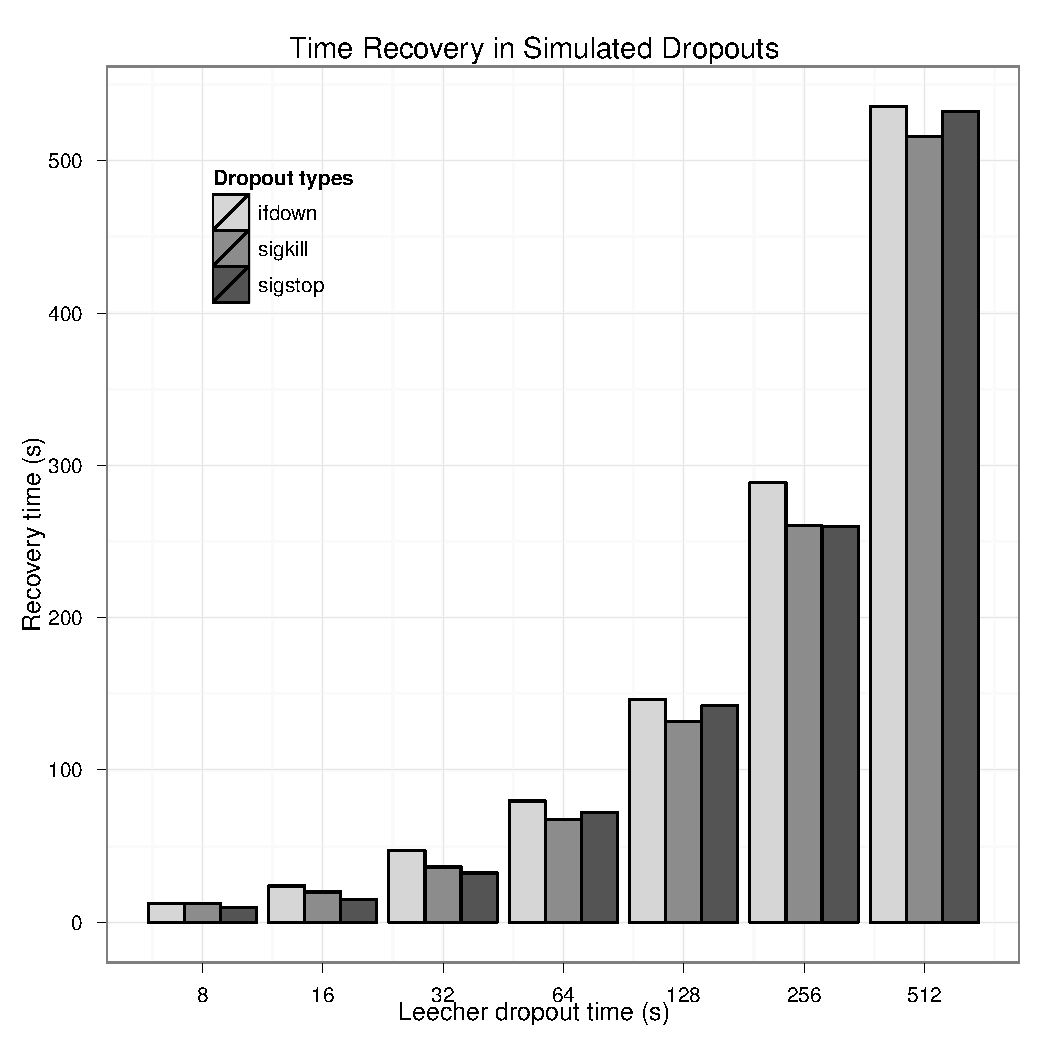
\includegraphics[width=0.5\textwidth]{src/img/virt-infra/recovery-in-simulated-dropouts.pdf}
  \end{center}
  \caption{Timpul de recuperare în raport cu intervalul de cădere}
  \label{fig:virt-infra:time-recovery}
\end{figure}

Remarcăm, drept concluzie, că prima soluție (\textbf{ifdown}) dezactivează
interfața de rețea a peer-ului pentru a simula sfârșitul conexiunii.
Rezultatele au arătat că deși timpul de recuperare are același ordin de
mărime ca în celelalte cazuri, acesta este mai mare. În concluzie, această
metodă este cea mai potrivită pentru a simula căderile de conexiune datorate
eșecului rețelei.

A doua soluție (\textbf{suspend}) suspendă clienții în timpul căderii
simulate (folosind SIGSTOP) și îi repornește ulterior (folosind SIGCONT).
Deși suspendarea clienților nu este o acțiune uzuală, rezultatele au arătat
că această metodă este similară cu metoda \textbf{stop}, raportat la timpul
de recuperare. Într-un mediu unde suspendarea peer-ilor este mai ușor de
obținut decât oprirea lor, o astfel de soluție se poate dovedi a fi
potrivită și poate oferi rezultate realiste.

A treia soluție (\textbf{stop}) constă în oprirea (folosind SIGKILL) și
restartarea clienților. Această soluție, deși agresivă, este
considerată a fi cea mai bună aproximare a unui comportament realist al
unei căderi de conexiuni, deoarece peer-ii au în mod normal o dinamică
ridicată a intrării și ieșirii dintr-un swarm.

\section{Configurația implementată și scenariile experimentale}
\label{sec:virt-infra:setup-scenarios}

Infrastructura completă, folosind automatizare, virtualizare și mecanismul
de simulare a căderilor, permite implementarea automată și gestiunea
unei varietăți mari de scenarii Peer-to-Peer. Fiecare gazdă virtualizată
OpenVZ rulează un singur client BitTorrent (sau tracker) și colectează
informații relevante pentru o analiză ulterioară. Stația commander
definește configurația noului scenariu și apoi îl rulează deasupra
infrastructurii virtualizate. Limitările de lățime de bandă, tipurile
de client, porturile folosite, rata de churn și fișierele torrent sunt
configurate pentru scenariul dat.

Un astfel de experiment simulează swarm-uri formate dintr-un singur
seeder și 39 de leecheri inițiali. 19 leecheri sunt peer-i cu o lățime
de bandă mare (512KB/s viteză de download, 256KB/s viteză de upload)
și 20 de leecheri sunt peer-i cu o lățime de bandă redusă (64KB/s viteză
de download, 32KB/s viteză de upload).

Timpul total al unei instanțe experimentale folosind toți cei 40 de peer-i
și o imagine CD de 700MB durează aproximativ 4 ore. Durează doar aproximativ
o jumătate de oră pentru clienții cu lățime de bandă mare să o descarce.

Am folosit unealta Linux Traffic Control (\texttt{tc}) combinată cu
opțiunea iptables set-mark pentru a limita traficul de la și către un VE.

\subsection{Experimentele de evaluare a performanței}

Configurația experimentală a folosit în acest caz doar șase noduri fizice
din cadrul infrastructurii. Cea mai mare parte a experimentelor au constat
în sesiuni simultane de descărcare. Fiecare sistem a rulat câte un client
anume, toate VE-urile rulând simultan și în aceleași condiții. Rezultatele
și datele de jurnalizare au fost colectate după ce fiecare client și-a
completat download-ul.

\subsection{Rezultate}

\begin{table}[ht]
  \centering
  \begin{tabular}{@{}lrrrr@{}}
    \toprule
    & \textbf{Test1} & \textbf{Test2} & \textbf{Test3} &
    \textbf{Test4} \\
    \midrule
    mărimea fișierului & 908MB & 4.1GB & 1.09GB & 1.09GB	\\
    seederi & 2900 & 761 & 521 & 496	\\
    leecheri & 2700 & 117 & 49 & 51	\\
    \midrule
    \textbf{Client} & \multicolumn{4}{c}{Timp de descărcare (secunde)} \\
    \midrule
    aria2c & 4620 & 3233 & 580 & 623 \\
    azureus & 1961 & 2313 & N/A & 420 \\
    bittorrent & 17580 & 3639 & 1560 & 840 \\
    libtorrent & \textbf{581} & \textbf{913} & \textbf{150} & \textbf{134} \\
    transmission & 2446 & 3180 & 420 & 300 \\
    tribler & 2040 & 1260 & N/A & N/A \\
    \bottomrule
  \end{tabular}
  \caption{Rezultatele swarm-urilor test}
  \label{table:virt-infra:testsw}
\end{table}

Tabelul~\ref{table:virt-infra:testsw} prezintă o comparație a clienților
BitTorrent testați în patru scenarii diferite. Fiecare scenariu se referă
la un swarm diferit. Deși a fost colectată o cantitate mare de date, doar
timpul total de descărcare este prezent în tabel.
